%!TEX root = draft.tex

\section{Reference Implementation}
\label{sec:reference implementation}

In this section, we propose an abstract implementation called reference implementation, which will be used as specification in simulation proof of later section.


\subsection{Reference Implementation Definition}
\label{subsec:reference implementation definition}

Given a specification $Spec$, its reference implementation is given as an tuple $RImp(Spec) = (Q,\Sigma,q_0,\rightarrow,li,correct)$, where

\begin{itemize}
\setlength{\itemsep}{0.5pt}
\item[-] Each state $(O,ro,del,arb,vis) \in Q$ contains five tuples. Here $O$ is a set of update operations, and we assume that no two operations in $O$ have same operation identifier. $ro$ is the replica order over operations in $O$. $del \subseteq (O \times O) \cup (O \times \mathbb{R})$ is the deliver order. $(o_1,o_2) \in del$ represents that the effect of $o_1$ is delivered to the replica of $o_2$ before $o_2$ happens, while $(o,r) \in del$ represents that the effect of $o$ is delivered to replica $r$ after the time point of the last operation of replica $r$. we require $del$ to only relate operations with different replica identifier. $arb \subseteq O \times O$ is the arbitration order.

    $vis = del \cdot ro$ is the visibility relation. $(o_1,o_2) \in vis$ represents that the effect of $o_1$ is visible to $o_2$, while $(o,r)$ represents that the effect of $o$ becomes visible to replica $r$ after the time point of the last operation of replica $r$. We require $vis$ to be acyclic and irreflexive, and $vis^{-1}$ to be finite. 

\item[-] $correct: Q \rightarrow \{ \textit{true},\textit{false} \}$ is a predicate. {\color {red} We consider only states of $Q$ that satisfy $correct$.}   

\item[-] $\Sigma = \Sigma_1 \cup \Sigma_2$ is the set of transition labels, where $\Sigma_1 = \{ (m,a,b,r,ar) \vert m \in \mathbb{M}, a,b \in \mathbb{D}, r \in \mathbb{R},$ $ar$ is an arbitration order $\}$ and $\Sigma_2 = \{ addDel(o,r) \vert o \in \mathbb{O}, r \in \mathbb{R} \}$.

\item[-] $li$ is a function that maps $q = (O,ro,del,arb,vis) \in Q$, $r \in \mathbb{R}$ and $o \notin O$ into a tuple $( O_l ,<_l, <_{\textit{l-arb}} )$. $li$ give local interpretation only for the time point when $o$, a new operation, will happen at the latest time point of some replica. Here $O_l = \{ vis^{-1}(o) \vert o$ is of replica $r \} \cup vis^{-1}(r)$, $<_{\textit{l-arb}}$ is a partial order over $O_1 \cup \{ o \}$, and $<_l \subseteq vis \uparrow_{(O_l,O_l)}$. $<_{\textit{l-arb}}$ is obtained from $arb \uparrow_{O_l \times I_l}$ by possibly adding some relation from operations between $I_l$ and $o$, and  between $o$ and $I_l$. we also require that

    \begin{itemize}
    \setlength{\itemsep}{0.5pt}
    \item[-] $<_l \subseteq vis \uparrow_{(O_l \times O_l)}$. If $o_1,o_2 \in O_l$, $(o_1,o_2) \in vis$ via $o'_1,\ldots,o'_m$, and $o'_1,\ldots,o'_m \in O_l$, then $(o_1,o_2) \in <_l$.

    \item[-] $<_l$ is determined by $vis$ over $O_l$. Therefore, $\forall r_1,r_2 \in \mathbb{R}$, if $\{ vis^{-1}(o) \vert o$ is of replica $r_1 \} \cup vis^{-1}(r_1)$ and $\{ vis^{-1}(o) \vert o$ is of replica $r_2 \} \cup vis^{-1}(r_2)$ contain same set of operations, then their corresponding $<_l$ is the same.
    \end{itemize}

\item[-] $\rightarrow \subseteq Q \times \Sigma \times Q$ is the transition relation. It contains three kinds of transitions: adding a deliver relation, doing a query operation, and doing an update operation.

    \begin {itemize}
    \item[-] Adding a deliver relation:

     $\begin{array}{l c} \bigfrac{o \in O, \neg(o \xrightarrow{vis} r)} {(O,ro,del,arb,vis) {\xrightarrow{addDel(o,r)}} (O,ro,del \cup \{ (o,r) \},arb,(del \cup \{ (o,r) \}) \cdot ro)} \end{array}$

    \item[-] Doing a query operation: Let $m$ be a query method.

     $\begin{array}{l c} \bigfrac{ o=(m(a,b),rid,oid) \notin O, \exists O', li((O,ro,del,arb,vis),r,o) = (O',\_,arb \uparrow_{O'}) \in Spec(m(a,b))} {(O,ro,del,arb,vis) {\xrightarrow{m(a,b,r,arb)}} (O,ro,del,arb,vis)}  \end{array}$

     \item[-] Doing an update operation: Let $m$ be an update method, {\color {red}let $arb'$ be obtained from $arb$ by (1) adding operation $o$, (2) adding possibly relations between operation of $arb$ and $o$, and (3) adding possibly relations between $o$ and operations of $arb$.}

     $\begin{array}{l c} \bigfrac{o = (m(a,b),r,oid) \notin O, \exists O', li((O,ro,del,arb,vis),r,o) = (O',\_,arb' \uparrow_{(O' \cup \{ o \})}) \in Spec(m(a,b))} {(O,ro,del,arb,vis) {\xrightarrow{m(a,b,r,arb')}} (O \cup \{ o \},ro \oplus o ,del \oplus o,arb',(del \oplus o) \cdot (ro \oplus o))}  \end{array}$

     $ro \oplus o = ro \cup \{ (o',o) \vert o'$ is of replica $r \}$ and $del \oplus o$ is obtained from $del$ by transforming each $(o',r)$ in $del$ into $(o',o)$. We further require that the candidate of operation identifier of $o$ is unique.
    \end{itemize}

\item[-] $q_0=(\emptyset,\emptyset,\emptyset)$ is the initial state.
\end{itemize}

\noindent {\bf Example 3. $RImp(S_{\textit{ORS}})$}: $li$ and $correct$ is defined as follows:

\begin{itemize}
\setlength{\itemsep}{0.5pt}
\item[-] Given $q = (O,ro,del,arb,vis)$, $r \in \mathbb{R}$ and $o \notin O$, $li(q,r,o) = ( O_l ,<_l, <_{\textit{l-arb}} )$. Here $<_{\textit{l-arb}} = \emptyset$.

$<_l = vis \uparrow_{(O_l \times O_l)} - \{ (o_1,o_2) \vert o_2 \notin Minus(q,o_1), \exists o_3, o_1 {\xrightarrow{vis}} o_3 {\xrightarrow{vis}} o_2, o_1$ and $o_2$ are visible to replica $r$ or operation of replica $r$, $o_3$ is not visible to replica $r$ nor operation of replica $r\}$.

Here $Minus(q,o_1)$ is defined as follows: (1) if $cont(o_1)=add(a,\top)$, then $Minus(q,o_1) = \{o_2 \vert cont(o_2)=rem(\top,a), o_1 {\xrightarrow{vis}} o_2, \neg \exists o_3,$ such that $( cont(o_3) = rem(\top,a) ) \wedge ( o_1 {\xrightarrow{vis}} o_3 {\xrightarrow{vis}} o_2 ) \}$, (2) otherwise, $Minus(q,o_1) = \emptyset$.

\item[-] $correct((O,ro,del,arb,vis))$ holds, if 

    \begin{itemize}
    \setlength{\itemsep}{0.5pt}
    \item[-] $\forall o \in O$, if $cont(o)=rem(\top,a)$, then $\exists o', cont(o')=add(a,top) \wedge o \in Minus(q,o')$. 
    
    \item[-] $arb= \emptyset$. 
    \end{itemize}
\end{itemize}

\noindent {\bf Example 4. $RImp(S_{\textit{list}})$}: $li$ and $correct$ is defined as follows:

\begin{itemize}
\setlength{\itemsep}{0.5pt}
\item[-] Given $q = (O,ro,del,arb,vis)$, $r \in \mathbb{R}$ and $o \notin O$, $li(q,r,o) = ( O_l ,<_l, <_{\textit{l-arb}} )$. Here $<_l = vis \uparrow_{(O_l \times O_l)}$. $<_{\textit{l-arb}}$ is as follows: (1) if $o$ is an $add$ operation, then $<_{\textit{l-arb}}$ is a total generated by adding $o$ into some place of $arb$, (2) otherwise, $<_{\textit{l-arb}} = arb$.

\item[-] $correct((O,ro,del,arb,vis))$ holds, if

    \begin{itemize}
    \setlength{\itemsep}{0.5pt}
    \item[-] Given $(O,vis,arb)$, we can go through operations of $O$ by first investigate minimal (w.r.t $vis$) operations, and then their immediate successors (w.r.t $vis$), and so on. During this process, for each operation $o$, we require $o$ to be correct similarly as in case of Example 2.

    \item[-] $arb$ is a acyclic total order over $add$ operations of $O$. 
    \end{itemize}
\end{itemize}

It is obvious that $RImp(Spec)$ is deterministic. Since $li$ and $cor$ are only used to define transition relation, when the context is clear, we could ignore these two tuples and write $RImp(Spec) = (Q,\Sigma,q_0,\rightarrow)$. The set of executions of $RImp(Spec) = (Q,\Sigma,q_0,\rightarrow)$, denoted $\llbracket RImp(Spec) \rrbracket$, is the set of all executions starts from $q_0$. Formally, $t = \alpha_1 \cdot \ldots \in \llbracket RImp(Spec) \rrbracket$, if there exists $q_1,\ldots \in Q$, such that $q_0 {\xrightarrow{\alpha_1}} q_1 {\xrightarrow{\alpha_2}} \ldots$.

Given an execution $t = \alpha_1 \cdots \in \llbracket RImp(Spec) \rrbracket$, its abstract trace $absT(t) = (O,<_{\textit{ro}},<_{\textit{vis}},<_{\textit{arb}})$ is generated as follows: Let $q_1,\ldots \in Q$ be the set of states, such that $q_0 {\xrightarrow{\alpha_1}} q_1 \ldots$.

\begin{itemize}
\setlength{\itemsep}{0.5pt}
\item[-] $O$ is the set of operations generated during $t$.

\item[-] $<_{\textit{ro}} = <_{r_1} \cup \ldots \cup <_{r_{\vert \mathbb{R} \vert}}$, where for each $i$, $<_i$ is the occurring order of operations with the $i$-th identifier in $\mathbb{R}$ over $t$.

\item[-] $(o_1,o_2) \in <_{\textit{vis}}$, if one of the following case holds: (1) $o_1$ is delivered into replica of $o_2$, and then $o_2$ happens, (2) $o_1$ and $o_2$ are of same replica and $o_1$ happens earlier than $o_2$.

\item[-] $<_{\textit{arb}}$ is the union of arbitration order of each $q_i$.
\end{itemize}

The following theorem states that the executions in $\llbracket RImp(Spec) \rrbracket$ are SRV consistent w.r.t $Spec$. Its proof can be found in Appendix \ref{sec:appendix definitions and proofs of section reference implementation}.

\begin{theorem}
\label{lemma:executions of reference implementation are SRV consistent}
$\forall t \in \llbracket RImp(Spec) \rrbracket$, $absT(t)$ is SRV consistent w.r.t $Spec$.
\end{theorem}


\noindent {\bf Reference Implementation with Causal Delivery}:

An operation $o_1$ happen-before \cite{Lamport:1978} an operation $o_2$, denoted $o_1 <_{hb} o_2$, if $o_1 {\xrightarrow{ (del \cup ro)^* }} o_2$. Causal delivery require that, for each pair of update operations $(o_1,o_2)$, if $o_1 <_{hb} o_2$, then for each replica $r$, $o_2$ can be delivered to replica $r$ if $o_1$ has already been delivered to replica $r$.

Given a specification $Spec$, its reference implementation with causal delivery is given as an tuple $RImp(Spec)_{\textit{cd}} = (Q,\Sigma,q_0,\rightarrow,li,cor)$. $RImp_{\textit{cd}}(Spec)$ can be obtained from $RImp(Spec)$ by only changing the transition rules of adding a delivery relation as follows:

\begin {itemize}
\setlength{\itemsep}{0.5pt}
\item[-] Adding a deliver relation:

$\begin{array}{l c} \bigfrac{o \in O, o \ is \ minimal \ w.r.t \ <_{hb} in \ \{ o' \vert (o',r) \notin vis, \forall o'' \in O \ with \ replica \ r, (o',o'') \notin vis \}} {(O,ro,del,arb,vis) {\xrightarrow{addDel(o,r)}} (O,ro,del \cup \{ (o,r) \},arb,(del \cup \{ (o,r) \}) \cdot ro)} \end{array}$

\end{itemize}

The following lemma states that $RImp(Spec)_{\textit{cd}}$ contains all the sequences of $RImp(Spec)$ that are causal delivery. Its proof can be found in Appendix \ref{sec:appendix definitions and proofs of section reference implementation}.

\begin{lemma}
\label{lemma:RImpcdSpec contains all the sequences of RImpSpec that are causal delivery}
$\llbracket RImp(Spec)_{\textit{cd}} \rrbracket = \{ t \vert t \in \llbracket RImp(Spec) \rrbracket \wedge t$ satisfies causal delivery $\}$.
\end{lemma}



\subsection{Compacted Reference Implementation}
\label{subsec:compacted reference implementation}

Let $RImp(Spec)^{op}$ be an LTS obtained from $RImp(Spec)$ by transforming each $(m,a,b,r,arb)$ transition into $(m,a,b,r)$ transition, and transforming each $addDel(o,r)$ transition into $\epsilon$ transition. Two states $q_1,q_2$ of $RImp(Spec)$ are equivalent, if they are weak bisimular on $RImp(Spec)^{op}$.

Given a state $q'=(O',ro',del',arb',vis')$ and $o' \in O$, Let $ip(o')$ be the immediate predecessor of $o'$ w.r.t $ro'$ in $q'$, $is(o')$ be the immediate successor of $o'$ w.r.t $ro'$ in $q'$ and $S_{delTo}(o') = \{o'' \vert (o'',o') \in del' \}$. when we say we penetrate $o'$ from $q'$, we obtain a state $q''=(O'',ro'',del'',arb'',vis'')$ as follows:

\begin{itemize}
\setlength{\itemsep}{0.5pt}
\item[-] $O'' = O' - \{ o' \}$.

\item[-] $ro''$ is obtained from $ro'$ by removing pairs contain $o'$ and adding $(ip(o'),is(o'))$.

\item[-] $del''$ is obtained from $del'$ by removing pairs contain $o'$ and adding $\{ (o_1,is(o')) \vert o_1 \in S_{delTo}(o')\}$.

\item[-] $vis'' = del'' \cdot ro''$, and $arb'' = arb' \uparrow_{O''}$.
\end{itemize}

Given a plus-minus specification $Spec$ and a state $q=(O,ro,del,arb,vis)$ of $RImp(Spec)$, given a plus operation $o \in O$, the set of minus operations for $o$ in $q$, denoted $Minus(q,o)$, is a set of minus operations of $O$. Intuitively, when an plus operations and its minus operations are seen by all replica, it should be equivalent to the case where this plus operation and its minus never happens. Formally,

\begin{itemize}
\setlength{\itemsep}{0.5pt}
\item[-] Let $S_p(q) = \{ o_1 \vert o_1$ is a plus operation, $\forall r \in \mathbb{R}, \exists o_2 \in Minus(q,o_1)$ such that $(o_2,r) \in vis$ or $(o_2,o_3) \in vis$ and $o_3$ is of replica $r\}$. $S_p(q)$ is the set of redundant plus operations of $q$.

\item[-] Let $S_m(q) = \{ o_1 \vert  \{ o_2 \vert o_1 \in Minus(o_2) \} \subseteq S_p(q) \}$. $S_m(q)$ is the set of redundant minus operations of $q$.

\item[-] Let $conc(q)$ be obtained from $q$ by penetrating operations in $S_p(q) \cup S_m(q)$ one by one.

\item[-] We require $q$ and $conc(q)$ to be equivalent.
\end{itemize} 

It is not hard to see that, the visibility among operations not penetrated remains the same after penetrating. Therefore, penetrating using different order lead to same consequence. 

\noindent {\bf Example 5. The case of OR-set}: We already give the definition of $Minus(q,o)$ of OR-set in Example 3. \figurename~\ref{fig:the process of penetrate operations of or-set} shows an example of erasing redundant operations. Here $+a_1$ (resp., $-a_1$) is an operation with content $add(a,\top)$ (resp., $rem(\top,a)$), and the subscript is used to distinguish different $add(a,top)$ operations. In \figurename~\ref{fig:the process of penetrate operations of or-set} (a), $+a_2$ is the redundant $add$ operation, and $-a_2$ is the redundant $rem$. We penetrate $+a_1$ from \figurename~\ref{fig:the process of penetrate operations of or-set} (a) to \figurename~\ref{fig:the process of penetrate operations of or-set} (b), while $ip(+a_2) = +f$, $is(+a_2) = +c$, and we explicitly color $S_{delTo}(+a_2)$ with blue color.  We penetrate $-a_2$ from \figurename~\ref{fig:the process of penetrate operations of or-set} (b) to \figurename~\ref{fig:the process of penetrate operations of or-set} (c). 


\begin{figure}[t]
  \centering
  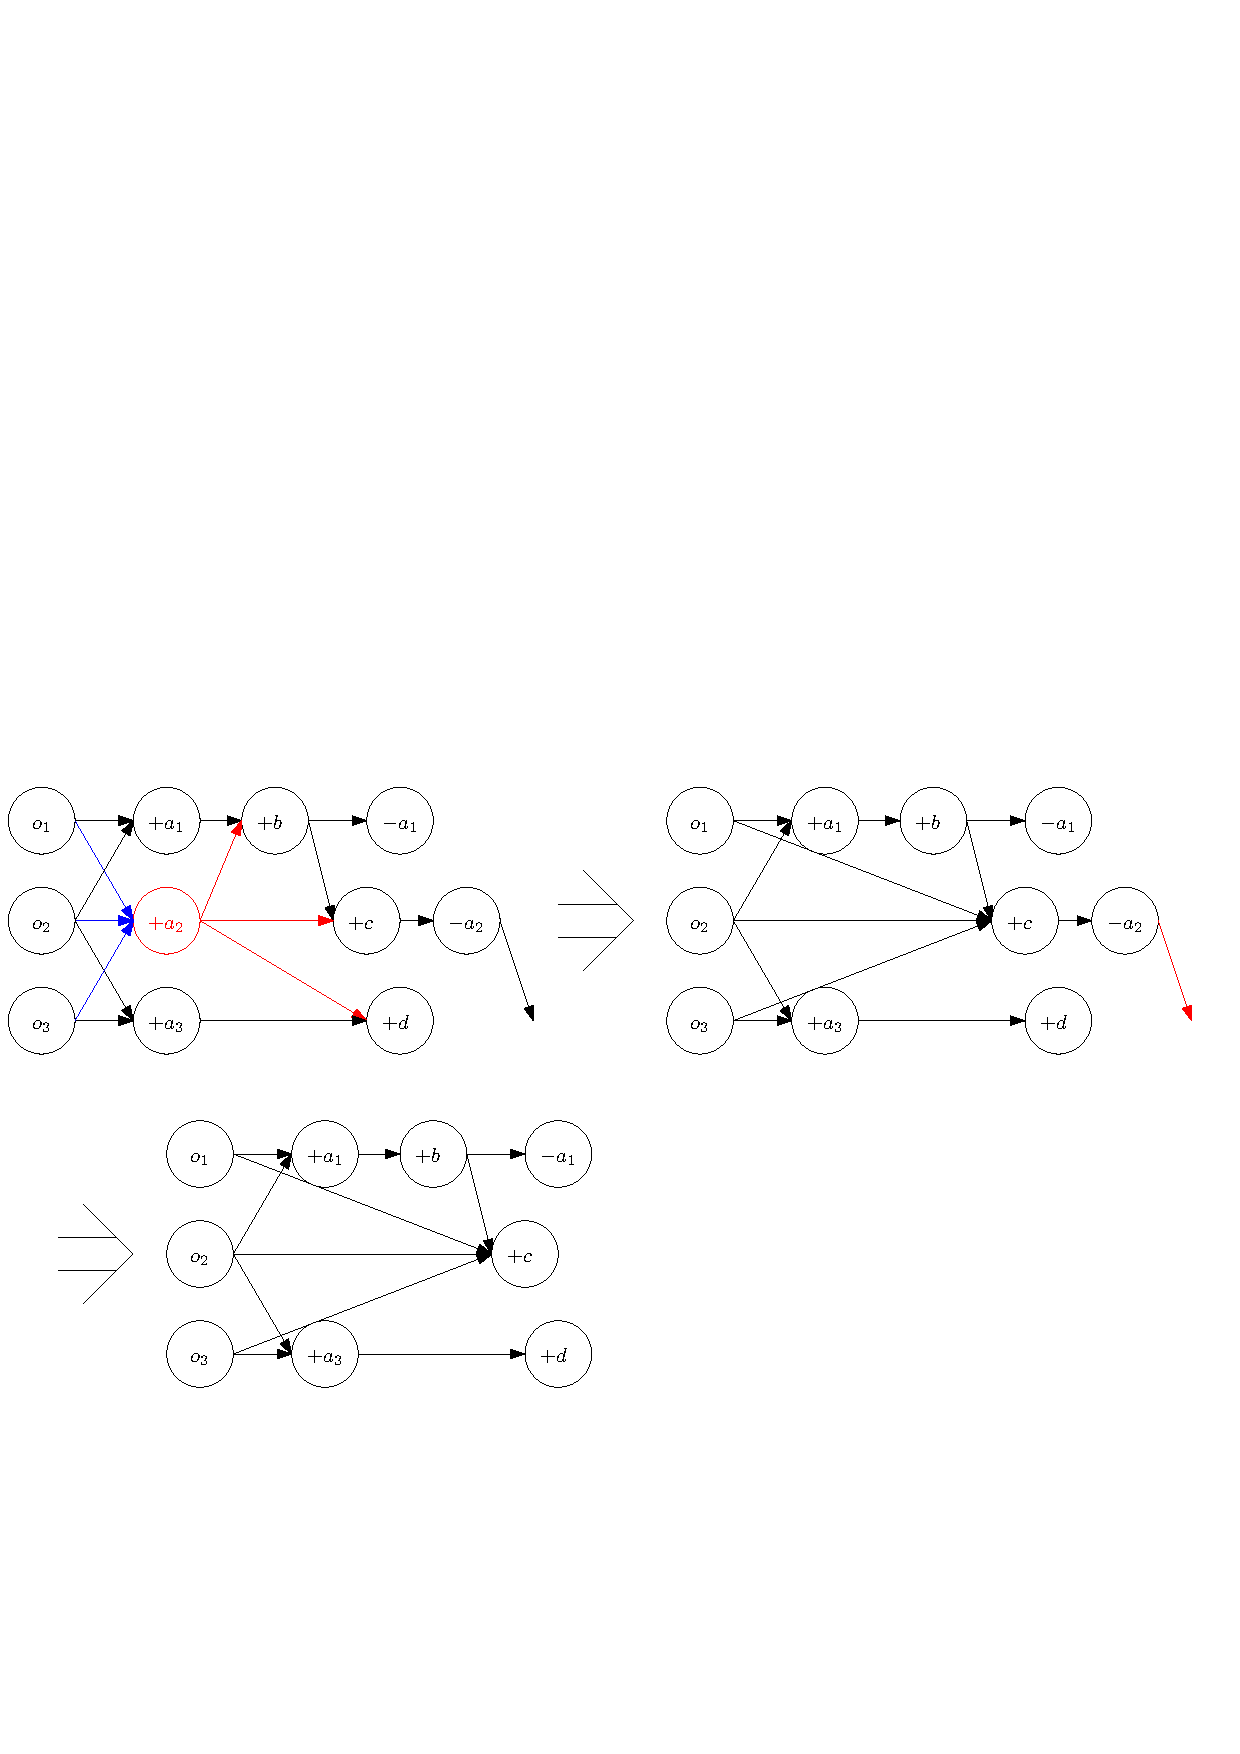
\includegraphics[width=0.85 \textwidth]{figures/PIC-Example-CompactProcess.pdf}
%\vspace{-10pt}
  \caption{The process of penetrating operations $+a_2$ and $-a_2$ of OR-set}
  \label{fig:the process of penetrate operations of or-set}
\end{figure}


\noindent {\bf Example 6. The case of Distributed list}: Given $q=(O,ro,del,arb,vis)$ and add operation $o$ where $cont(o)=add(a,\_,\top)$, $o' \in Minus(q,o)$, if (1) $cont(o')=rem(pos,a)$, and (2) Recall that we have already check the correctness of operations of $(O,vis,arb)$ as in Example 2. When we comes to $o'$ in this process, $seq(o')[pos]=o$. 

\figurename~\ref{fig:the process of penetrate operations in distributed list} shows an example of distributed list. Here $o_1 = add(a,1,\top)$, $o_2 = add(b,1,\top)$, $o_3 = add(c,2,\top)$, $o_4 = add(c,2,\top)$, $o_5 = add(d,3,\top)$, and the arbitration order is $o_1 {\xrightarrow{arb}} o_4 {\xrightarrow{arb}} o_3 {\xrightarrow{arb}} o_2 {\xrightarrow{arb}} o_5$. In \figurename~\ref{fig:the process of penetrate operations in distributed list} (a), $o_3$ is the redundant $add$ operations, and $rem(2,c)$ and $rem(3,c)$ are the redundant $rem$ operations. After penetrating $o_3$, $rem(2,c)$ and $rem(3,c)$, we obtain \figurename~\ref{fig:the process of penetrate operations in distributed list} (b). 

\begin{figure}[t]
  \centering
  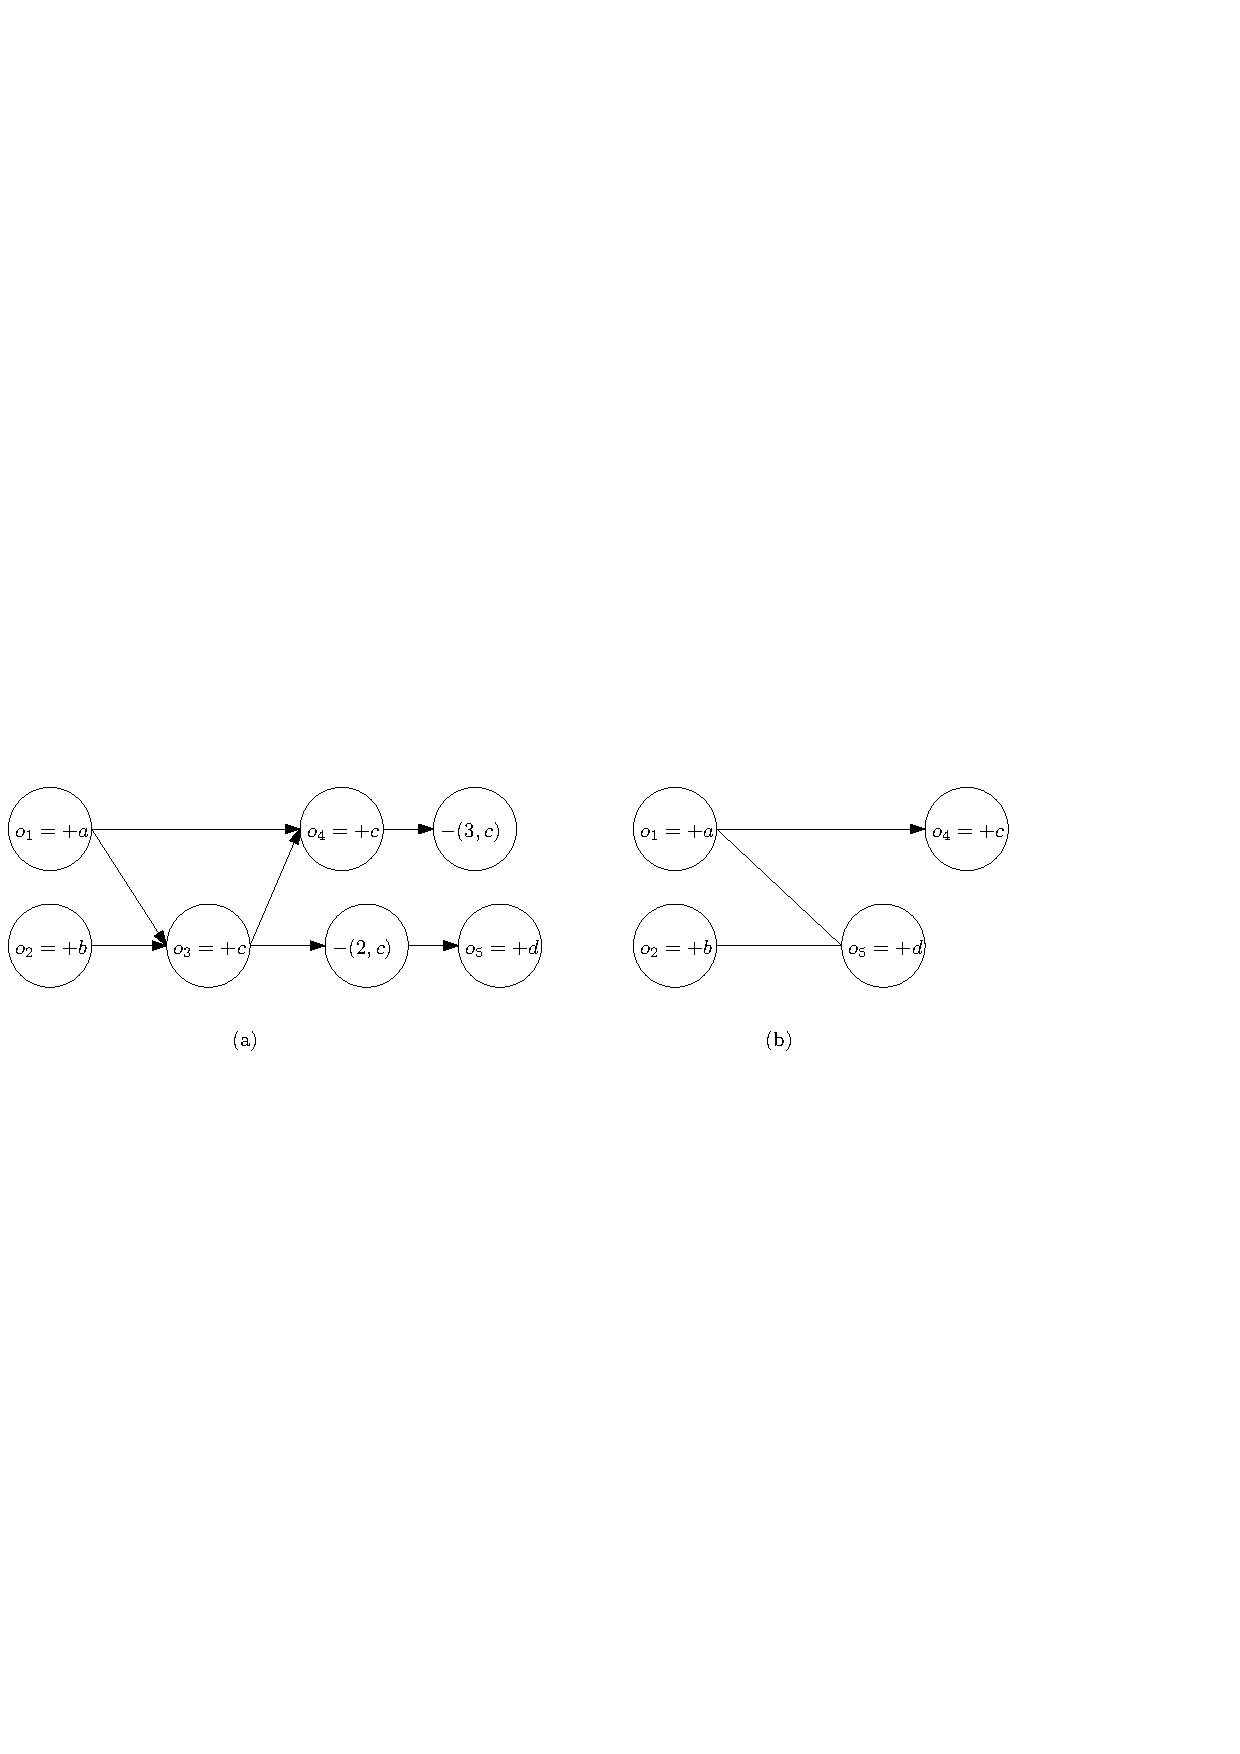
\includegraphics[width=0.7 \textwidth]{figures/PIC-Example-CompactProcess-list}
%\vspace{-10pt}
  \caption{The process of penetrating operations of distributed list}
  \label{fig:the process of penetrate operations in distributed list}
\end{figure}

Note that, in the case of OR-set, given $rem$ operation $o_r$, $\vert \{ o_a \vert o_r \in Minus(o_a) \} \vert$ may be larger than $1$; while in the case of distributed list, given $rem$ operation $o_r$, $\vert \{ o_a \vert o_r \in Minus(o_a) \} \vert = 1$. 

Given a plus-minus specification $Spec$, its compacted reference implementation is given as an tuple $CRImp(Spec) = (Q,\Sigma,q_0,\rightarrow,li,correct)$. $CRImp(Spec)$ can be obtained from $RImp(Spec) = (Q',\Sigma,q_0,\rightarrow',li,correct)$ as follows: 

\begin{itemize}
\setlength{\itemsep}{0.5pt}
\item[-] $Q \subseteq Q'$. $\forall o \in Q$, $q = conc(q)$. 

\item[-] If $\alpha = addDel(\_,\_)$: $q_1 {\xrightarrow{\alpha}} q_2$, if $\exists q_3$, such that $q_1 {\xrightarrow{\alpha}}' q_3 \wedge q_2 = conc(q_3)$. 

\item[-] If $\alpha=m(\_,\_,\_,\_)$ and $m$ is a query method: $q_1 {\xrightarrow{\alpha}} q_2$, if $q_1 {\xrightarrow{\alpha}}' q_2$. 

\item[-] If $\alpha=m(a,b,r,arb)$ and $m$ is an update method: $q_1 {\xrightarrow{m(a,b,r,arb)}} q_2$, if $\exists q_3,arb'$, such that $q_1 {\xrightarrow{m(a,b,r,arb')}}' q_3 \wedge q_2 = conc(q_3)$. 
\end{itemize} 








Given an execution $t = \alpha_1 \cdots \in \llbracket RImp(Spec) \rrbracket$, its abstract trace $absT(t) = (O,<_{\textit{ro}},<_{\textit{vis}},<_{\textit{arb}})$ is generated as follows: Let $q_1,\ldots \in Q$ be the set of states, such that $q_0 {\xrightarrow{\alpha_1}} q_1 \ldots$.

\begin{itemize}
\setlength{\itemsep}{0.5pt}
\item[-] $O$ is the set of operations generated during $t$.

\item[-] $<_{\textit{ro}} = <_{r_1} \cup \ldots \cup <_{r_{\vert \mathbb{R} \vert}}$, where for each $i$, $<_i$ is the occurring order of operations with the $i$-th identifier in $\mathbb{R}$ over $t$.

\item[-] $(o_1,o_2) \in <_{\textit{vis}}$, if one of the following case holds: (1) $o_1$ is delivered into replica of $o_2$, and then $o_2$ happens, (2) $o_1$ and $o_2$ are of same replica and $o_1$ happens earlier than $o_2$.

\item[-] $<_{\textit{arb}}$ is the union of arbitration order of each $q_i$.
\end{itemize}













Let $poSet(\llbracket CRImp(Spec) \rrbracket)$ (resp., $poSet(\llbracket RImp(Spec) \rrbracket)$) be the sets of sequences obtained by using poset upon sequences in $\llbracket CRImp(Spec) \rrbracket$ (resp., $\llbracket RImp(Spec) \rrbracket$). The following lemma stats that $poSet(\llbracket CRImp(Spec) \rrbracket) = poSet(\llbracket RImp(Spec) \rrbracket)$. It is not hard to prove this since when defining transition relation of $CRImp(Spec)$ from that of $CRImp(Spec)$, we replace a state with a equivalent state. Its proof is obvious and omitted.

\begin{lemma}
\label{lemma:CRImpcdSpec and RImpcdSpec contain the same set of trace}
$poSet(\llbracket CRImp(Spec) \rrbracket) = poSet(\llbracket RImp(Spec) \rrbracket)$.
\end{lemma}

Similar as the case of reference implementation, we can add the restriction of causal-delivery into compacted reference implementation.

Given a plus-minus specification $Spec$, its compacted reference implementation with causal delivery is given as an tuple $CRImp_{cd}(Spec) = (Q,\Sigma,vis,q_0,li,\rightarrow_{cd},livReq)$. $CRImp_{cd}(Spec)$ can be obtained from $CRImp(Spec) = (Q,\Sigma,vis,q_0,li,\rightarrow_c,livReq)$ by only changing the transition rules of delivering operations as follows: $\rightarrow_{cd} = \{ q_1 {\xrightarrow{addDel(o,r)}}_{cd} q_2 \vert q_1 {\xrightarrow{addDel(o,r)}}_c q_2 \wedge$ $o$ is minimal w.r.t $<_{hb}$ among operations not visible to replica $r$ in $q_1 \}$.

It is easy to see that $CRImp_{cd}(Spec)$ contains all the traces of $CRImp(Spec)$ that are causal delivery, as stated by the following lemma. Its proof is obvious and omitted.

\begin{lemma}
\label{lemma:CRImpcdSpec contains all the traces of CRImpSpec that are causal delivery}

$\llbracket CRImp(Spec)_{cd} \rrbracket = \{ t \vert t \in \llbracket CRImp(Spec) \rrbracket \wedge t$ satisfies causal delivery $\}$.
\end{lemma}
























\forget
{
\section{Reference Implementation}
\label{sec:reference implementation}

In this section, we propose an abstract implementation called reference implementation, which will be used as specification in simulation proof of later section.


\subsection{Reference Implementation Definition}
\label{subsec:reference implementation definition}

An labeled transition system (LTS, for short) is a tuple $A = (Q,\Sigma,\rightarrow,q_0)$, where $Q$ is a set of states, $\Sigma$ is an alphabet of transition labels, $\rightarrow \subseteq Q \times \Sigma \times Q$ is a transition relation and $q_0$ is the initial state. In this paper, the specification and the semantics of CRDT implementation will be modelled as LTS. Then, checking eventual consistency is a instance of a more general notion of refinement between LTS where only actions in a specific alphabet $\Sigma$ is observable. It has been shown that refinement is equivalent to the existence of backward simulations, modulo the addition of history variables that record events in the implementation, and to the existence of forward simulations provided that the right-hand side LTS B is $\Sigma$-deterministic \cite{Abadi:1991,Lynch:1995}. In this paper we focus on proofs based on forward simulations because they are easier to automatize, and we need to ensure that reference implementations are deterministic.

In this paper, we focus on operation-based CRDT algorithm, where each operation is done locally (without communication between replicas), and when a replica does a update operation, it will broadcast the operation to all other replica. Here we assume the set of replica identifier is already fixed into $RId=\{1,\ldots,n\}$.

The operations of a CRDT are divided into two kinds: query operation and update operation.

\begin{itemize}
\setlength{\itemsep}{0.5pt}
\item[-] A query operation is used only for reading the content of ``abstract state'' and does not influence ``abstract state''. Or we can say, if $(A,<) \in Spec(o)$ for some and $A' \subseteq A$ is obtained from $A$ by erasing some query operations, then $(A',< \cap (A' \times A')) \in Spec(o)$.

    We require query method to be happen unconditionally. Or we can say, if $m$ is a query method, then the union of $Spec(m,\_,\_)$ is $PoSet_{\Sigma(M,D)}$.

\item[-] A update operation influences ``abstract state'' while it does not return value. {\color {red}Note that in some case, a update operation can happen if some condition is satisfied, such as $ins(itm,pos)$ of distributed list. However, this can be done by checking if its local interpretation is in the specification.}
\end{itemize}

%Let $qry(M,D,RId,OId)$ (resp., $upd(M,D,RId,OId)$) be the set of query operations (resp., update operations) using method in $M$, arguments and return values in $D$, replica identifiers in $RId$ and operation identifiers in $OId$.

Given a specification $Spec$, its reference implementation is given as an tuple $RImp(Spec) = (Q,\Sigma,vis,q_0,li,\rightarrow,livReq)$, where

\begin{itemize}
\setlength{\itemsep}{0.5pt}
\item[-] Each state $(uO,ro,del) \in Q$ contains three tuples. Here $uO$ is a set of update operations, $ro$ is the replica order among operations in $uO$, and $del \subseteq (uO \times uO) \cup (uO \times RId)$ is the deliver order. $(o_1,o_2) \in del$ represents that the effect of $o_1$ (its message) is delivered to the replica of $o_2$ just before the time point $o_2$ happens. $(o,r) \in del$ represents that the effect of $o$ is delivered to replica $r$ after the time point of the last operation of replica $r$. We require that $(ro \cup del)^*$ being acyclic and irreflexive. %$(ro \cup del)^{*-1}$ to be finite,
    and we require $del$ to only relate operations with different replica identifier. We assume that $uO$ does not contain two operations with the same identifier. Note that we only record update operations in state. \footnote{{\color {red}We require that the tuple of $Q$ contain enough information for checking correctness of operations. Sometimes, if $Spec$ use additional information to check correctness of operations, $Q$ should contain more information. For example, to deal with distributed list specification \cite{Attiya:2016}, a list order is added to tuples of $Q$. Similarly, when needed, we add more information into $\Sigma$ and extended the transition relation $\rightarrow$.}}

\item[-] $\Sigma = \Sigma_{op} \cup \Sigma_{del}$ is the set of transition labels. Here $\Sigma_{op}$ is the set of operations using method in $M$, arguments and return values in $D$, and replica identifiers in $RId$. %and operation identifiers in $OId$.
    $\Sigma_{del}=\{ addDel(o,r) \vert o \in OId, r \in RId \}$.

\item[-] $vis : Q \rightarrow (uO \times uO) \cup (uo \times RId)$ is the visibility relation. $vis$ is irreflexive and acyclic. $(o_1,o_2) \in vis$ represents that the effect of $o_1$ is visible to $o_2$. $(o,r)$ represents that the effect of $o$ become visible to replica $r$ after the time point of the last operation of replica $r$.

    Since we are dealing with operation-based CRDT, we fix $vis$ relation to be $del \cdot ro$.

\item[-] $li: Q \times RId \rightarrow PoSet_{\Sigma(M,D)}$ is a function that maps each replica identifier into a poset of operations. Note that, we do not give local interpretation for each operation in $uO$. The reason is that intuitively, CRDT algorithms do not have speculative execution and it is enough to give local interpretation for the newest operation of each replica, and keep the local interpretation of other operations unchanged. we explain how to achieve this below.

    Here we leave enough freedom for defining different local interpretation for different algorithms. The only requirements to $li(q,r) = (O_{li},<_{li},l_{li})$ is:

    \begin{itemize}
    \setlength{\itemsep}{0.5pt}
    %\item[-] The union of local interpretation of each replica is acyclic.
    \item[-] $O_{li}$ contains all operations visible to replica $r$.

    \item[-] $<_{li}$ is a subset of $vis_q$ of replica $r$ and is constructed only upon $ro$ and $del$, where $vis_q$ is the visibility relation of $q$. Moreover, we require that if $o_1,o_2 \in O_{li}$, $o_1$ is visible to $o_2$ via $o'_1,\ldots,o'_m$, and $o'_1,\ldots,o'_m \in O_{li}$, then $(o_1,o_2) \in <_{li}$. Here we say $o_1$ is visible to $o_2$ via $o'_1,\ldots,o'_m$, if one of the following cases holds: (1) $o'_1$ (resp., $o'_{\textit{i+1}}$, $o_2$)is the immediate successor of $o_1$ (resp., $o'_i$, $o'_m$) w.r.t $ro$, or (2) $(o_1,o'_1) \in del$, $o'_{\textit{i+1}}$ (resp., $o_2$)is the immediate successor of $o'_i$ (resp., $o'_m$) w.r.t $ro$.

    \item[-] $l_{li}$ is a labeling function that maps each operation $(m,a,b,ird,oid)$ into $(m,a,b)$.
    \end{itemize}

\item[-] $\rightarrow \subseteq Q \times \Sigma \times Q$ is the transition relation. It contains three kinds of transitions: adding a deliver relation, doing a query operation, and doing an update operation.

    \begin {itemize}
    \item[-] Adding a deliver relation:

     $\begin{array}{l c} \bigfrac{o \in uO, \neg(o \xrightarrow{vis} r)} {(uO,ro,del) {\xrightarrow{addDel(o,r)}} (uO,ro,del \cup \{ (o,r) \})} \end{array}$

    \item[-] Doing a query operation: Let $m(a,b)$ be a query operation.

     $\begin{array}{l c} \bigfrac{li((uO,ro,del),r) \in Spec(m,a,b)} {(uO,ro,del) {\xrightarrow{m(a,b,r)}} (uO,ro,del)}  \end{array}$

     \item[-] Doing an update operation: Let $m(a,b)$ be an update operation.

     $\begin{array}{l c} \bigfrac{o = (m,a,b,r,oid) \notin uO, li((uO,ro,del),r) \in Spec(m,a,b)} {(uO,ro,del) {\xrightarrow{m(a,b,r)}} (uO \cup \{ o \},ro \oplus o ,del \oplus o)}  \end{array}$

     $ro \oplus o = ro \cup \{ (o',o) \vert o'$ is of replica $r \}$, $del \oplus o$ is obtained from $del$ by transforming each $(o',r)$ in $del$ into $(o',o)$.
    \end{itemize}

    %{\color {red}Note that, in query and update operation transition, we make operation to be argument. This is because that, in $livReq$, we need to check whether an operation has been delivered to a replica. When the context is clear, we may omit this argument.}

\item[-] $q_0=(\emptyset,\emptyset,\emptyset)$ is the initial state.

\item[-] With above tuple we could make each operation correct, while still unable to ensure $\textit{EVENTUAL}$ property in Definition \ref{definition:eventual consistency}. Let $\Sigma^{'\infty}$ be the set of finite and infinite sequences over $\Sigma'$. $livReq: (\Sigma_{op} \cup \Sigma_{del})^{ \infty } \rightarrow \{ \textit{true},\textit{false} \}$ is a predicate used to select only a subset of executions.

    Since we are dealing with operation-based CRDT, we fix $livReq$ to be that, $livReq(t) = \textit{true}$, if either $t$ is finite, {\color {red}or for each update operation $o$ introduced into some $uO$ during $t$ and each replica identifier $r$, $addDel(o,r) \in t$.} Or we can say, for each execution with infinite actions, we require each operation to be eventually delivered to each replica. We also assume that $t$ does not contain two operations with the same identifier.
\end{itemize}

The set of executions of $RImp(Spec) = (Q,\Sigma,vis,q_0,li,\rightarrow,livReq)$, denoted $\llbracket RImp(Spec) \rrbracket$, is the set of all executions starts from $q_0$ and conforms $livReq$. Formally, $t = \alpha_1 \cdot \ldots \in \llbracket RImp(Spec) \rrbracket$, if there exists $q_1,\ldots \in Q$, such that $q_0 {\xrightarrow{\alpha_1}} q_1 {\xrightarrow{\alpha_2}} \ldots$, and $livReq(t) = \textit{true}$.

Given an execution $t \in \llbracket RImp(Spec) \rrbracket$, its global interpretation $gi(t) \in PoSet_{\Sigma(M,D)}$ is its ``visibility relation'' among all of its operations and is formally defined as follows: $gi(t) = (O_{gi},<_{gi},l_{gi})$, where

\begin{itemize}
\setlength{\itemsep}{0.5pt}
\item[-] $O_{gi}$ is the set of operations of $t$. Or we could say, $O_{gi}$ is the set of operations introduced into some $uO$ during $t$.

\item[-] Assume $t = \alpha_1 \cdot \ldots$ and $\exists q_1,\ldots$, such that $q_0 {\xrightarrow{\alpha_1}} q_1 {\xrightarrow{\alpha_2}} \ldots$ and $livReq(t) = \textit{true}$. Let function $ord$ be a relation constructed as follows:

    \begin{itemize}
    \setlength{\itemsep}{0.5pt}
    \item[-] $ord(0) = \emptyset$.

    \item[-] If $\alpha_i = addDel(o,r)$, then $ord(i) = ord(i-1) \cup \{ (o,r) \}$.

    \item[-] If $\alpha_i = m(a,b,r)$ and let $o$ be the operation introduced into $uO$ because of $\alpha_i$ transition, then $ord(i) = ord(i-1) \cup \{ (o',o) \vert (o',r) \in ord(i-1) \vee (o',(\_,\_,\_,r,\_)) \in ord(i-1) \}$.
    \end{itemize}

    Then, $<_{gi} = (ord(1) \cup \ldots) - \{(o,r) \vert o \in OId, r \in RId\}$.

\item[-] $l_{gi}$ is a labeling function that maps each operation $(m,a,b,rid,oid)$ into $(m,a,b)$.
\end{itemize}

Given a sequence $t = \alpha_1 \cdots \in \llbracket RImp(Spec) \rrbracket$, let $poSet(t)=(O_t,<_t)$ be that: (1) $O_t$ is the set of operations of $t$, and (2) $<_t = <_{t1} \cup \ldots \cup <_{tn}$, where for each $i \in RId$, $<_{ti}$ is the projection of $t$ on operations of replica $i$. The following lemma states that, executions in $\llbracket RImp(Spec) \rrbracket$ are eventual consistent w.r.t $Spec$. Its proof can be found in Appendix \ref{subsec:appendix proof of lemma executions of reference implementation are eventual consistent}. To prove this lemma, for each operation $o$ which is first introduced by a transition from $q_i$ to $q_{i+1}$, the local interpretation of $o$ is chosen to be $li(q_i,r)$, where $r$ is the replica of $o$.

\begin{lemma}
\label{lemma:executions of reference implementation are eventual consistent}
$\forall t \in \llbracket RImp(Spec) \rrbracket$, $poSet(t)$ is eventual consistent w.r.t $Spec$.
\end{lemma}

Note that the opposite direction of this lemma does not hold: there may exists executions which is eventual consistent w.r.t $Spec$ but not in $\llbracket RImp(Spec) \rrbracket$.



\subsection{Reference Implementation with Causal Delivery}
\label{subsec:reference implementation with causal delivery}

According to \cite{Lamport:1978}, an operation $o_1$ happen-before an operation $o_2$, denoted $o_1 <_{hb} o_2$, if $o_1 {\xrightarrow{ (vis \cup ro)^* }} o_2$. Some CRDT algorithm use an assumption called causal delivery. Causal delivery require that, for each pair of update operations $(o_1,o_2)$, if $o_1 <_{hb} o_2$, then for each replica $r$, $o_2$ can be delivered to replica $r$ if $o_1$ has already been delivered to replica $r$.

Given a specification $Spec$, its reference implementation with causal delivery is given as an tuple $RImp_{cd}(Spec) = (Q,\Sigma,vis,q_0,li,\rightarrow,livReq)$. $RImp_{cd}(Spec)$ can be obtained from $RImp(Spec)$ by only changing the transition rules of delivering operations into follows:

\begin {itemize}
\setlength{\itemsep}{0.5pt}
\item[-] Adding a deliver relation:

$\begin{array}{l c} \bigfrac{o \in uO, o \ is \ minimal \ w.r.t \ <_{hb} \ among \ operations \ not \ visible \ to \ replica \ r} {(uO,ro,del) {\xrightarrow{addDel(o,r)}} (uO,ro,del \cup \{ (o,r) \})} \end{array}$

\end{itemize}

It is easy to see that $RImp_{cd}(Spec)$ contains all the traces of $RImp(Spec)$ that are causal delivery, as stated by the following lemma. Its proof is obvious and omitted.

\begin{lemma}
\label{lemma:RImpcdSpec contains all the traces of RImpSpec that are causal delivery}

$\llbracket RImp(Spec)_{cd} \rrbracket = \{ t \vert t \in \llbracket RImp(Spec) \rrbracket \wedge t$ satisfies causal delivery $\}$.
\end{lemma}



\subsection{Plus-Minus Specification and its Compacted Reference Implementation}
\label{subsec:plus-minus specification and its compacted reference implementation}

%Two states $q_1,q_2$ of $\llbracket RImp(Spec) \rrbracket$ are equivalent, if for each execution $t_1$ starts from $q_1$, there exists execution $t_2$ starts from $q_2$, such that $t_1$ and $t_2$ contains the same operation sequence.

Two states $q_1,q_2$ of $\llbracket RImp(Spec) \rrbracket$ are equivalent, if they are weak bisimilar on $\llbracket RImp(Spec) \rrbracket_o$, which is obtained from $\llbracket RImp(Spec) \rrbracket$ by transforming $addDel$ transitions into $\epsilon$ transitions.

A specification $Spec$ is said to be a plus-minus specification, if

\begin{itemize}
\setlength{\itemsep}{0.5pt}
\item[-] $Spec$ contains a query method called read and two update method called plus and minus. (They may use different name. For example, the plus method may be called insert or put, while the minus method may be called remove).

\item[-] Given a state $q = (uO,ro,del)$ of $\llbracket RImp(Spec) \rrbracket$ and a plus operation $o_p \in uO$, its direct-minus operations, denoted $dirM(o_p)$, is a set of minus operations. $dirM(o_p)$ satisfy the following requirements:

    \begin{itemize}
    \setlength{\itemsep}{0.5pt}
    \item[-] Let $ToPent_p(q)$ be the set of plus operations, such that $o \in ToPent_p$, if for each replica $r$, $\exists o' \in dirM(o)$ and $o'$ is visible to replica $r$ in $q$.

    \item[-] Let $ToPent_m(q) = \{ o \vert  \{ o' \vert o \in dirM(o') \} \subseteq ToPent_p \}$.

    \item[-] $q$ and $pent(q)$ are equivalent. Here $pent(q)$ is obtained from $q$ by ``penetrating operations in $ToPent_p(q)$ and $ToPent_m(q)$ one by one'' (explained below).
    \end{itemize}
\end{itemize}

Let us explain how to penetrate an operation $o$ in a state $q$. Let $o_{ip}(o)$ be the immediate predecessor of $o$ w.r.t $ro$, $o_{is}(o)$ be the immediate successor of $o$ w.r.t $ro$, $O_{to}(o) = \{o_1 \vert o_1 {\xrightarrow{ del }} o \}$ and $O_{from} = \{o_1 \vert o {\xrightarrow{ del }} o_1 \}$. To penetrate $o$ in $q$, we (1) remove $o$, $O_{to}$ and $O_{from}$ from $q$, and (2) add $o_{ip}(o) {\xrightarrow{ ro }} o_{is}(o)$ and $\{ o_1 {\xrightarrow{ ro }} o_{is}(o) \vert o_1 \in O_{to}(o)\}$.

\begin{figure}[t]
  \centering
  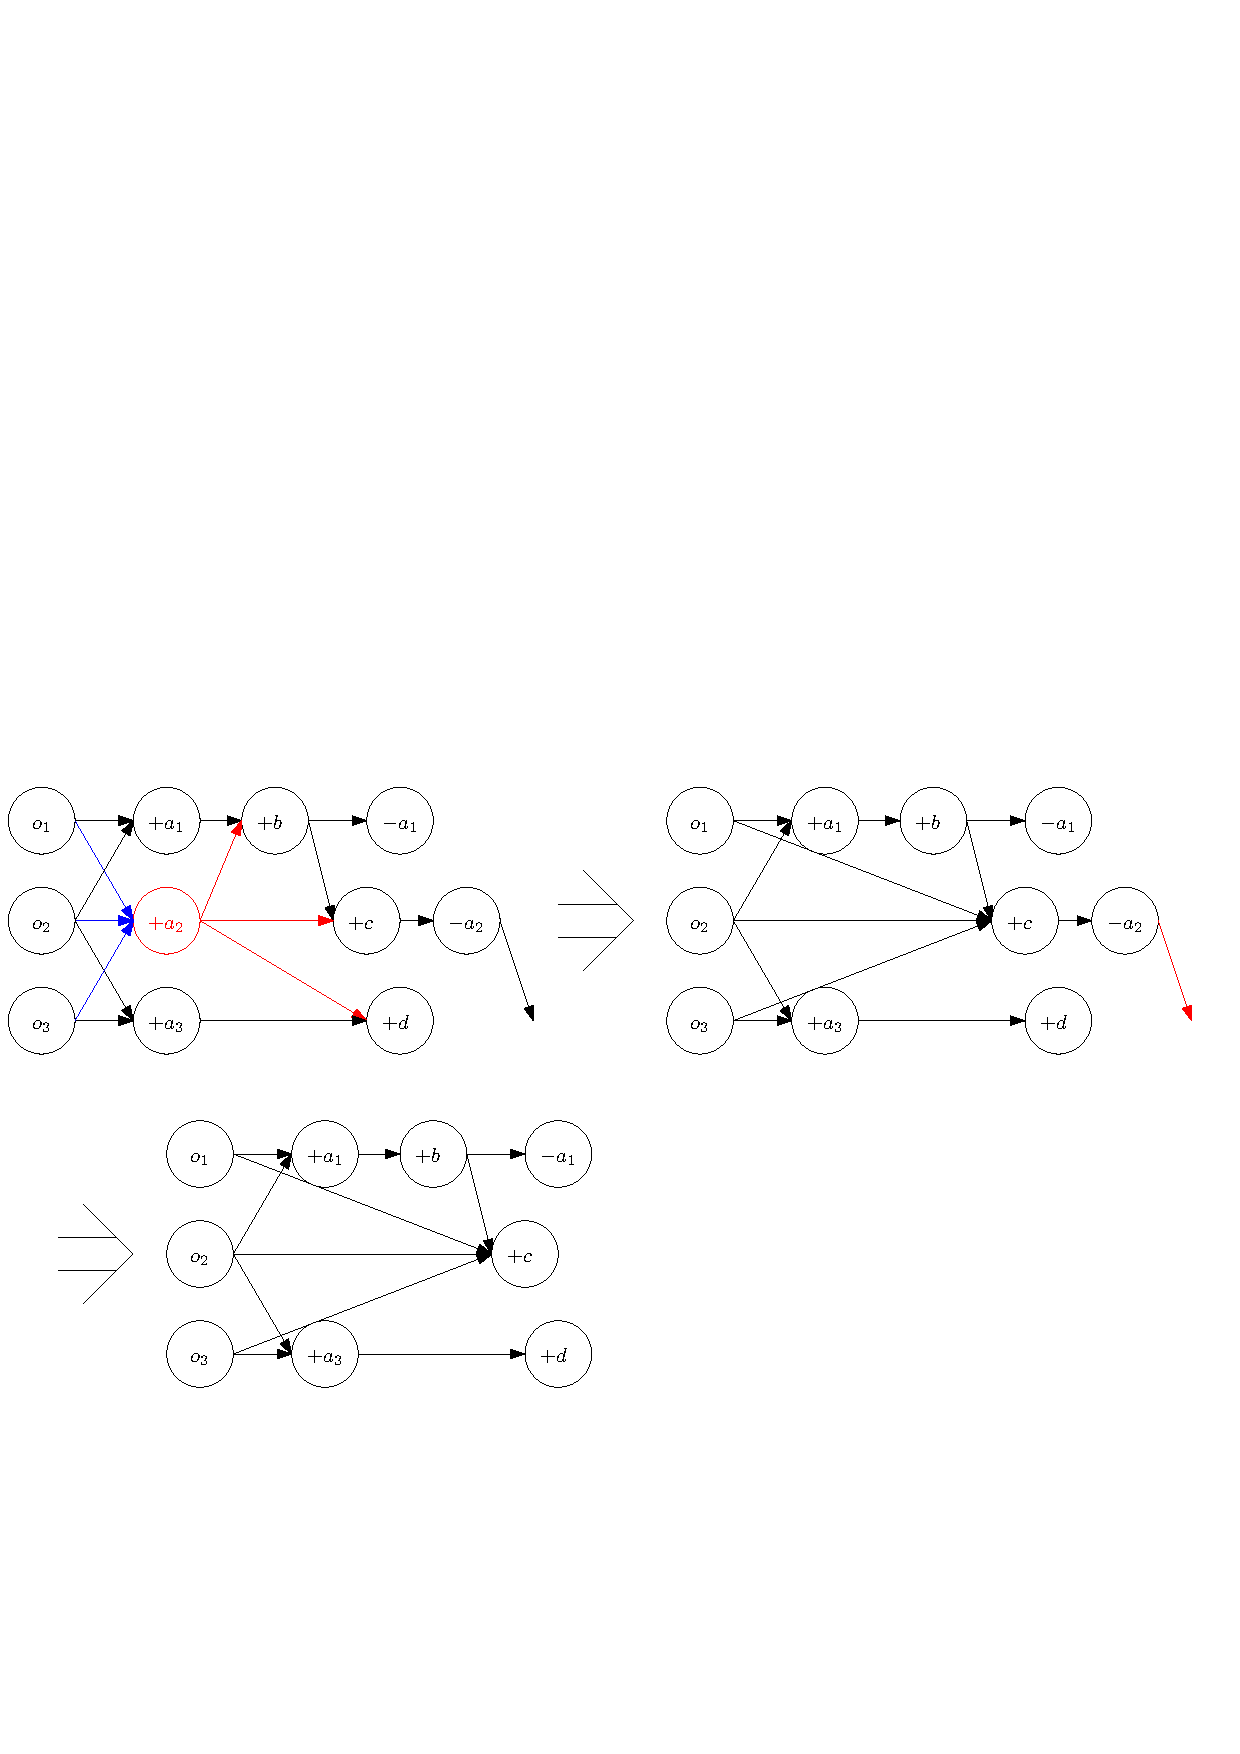
\includegraphics[width=0.8 \textwidth]{figures/PIC-Example-CompactProcess.pdf}
%\vspace{-10pt}
  \caption{The process of penetrating operations $+a_2$ and $-a_2$}
  \label{fig:the process of penetrate operations}
\end{figure}

\figurename~\ref{fig:the process of penetrate operations} shows an example of first penetrate $+a_2$ (from \figurename~\ref{fig:the process of penetrate operations} (a) to \figurename~\ref{fig:the process of penetrate operations} (b)) and then penetrate $-a_2$(from \figurename~\ref{fig:the process of penetrate operations} (b) to \figurename~\ref{fig:the process of penetrate operations} (c)). This is an practical example for the case of OR-set algorithm \cite{Shapiro:2011,Bieniusa:2012}. In \figurename~\ref{fig:the process of penetrate operations} (a), $o_{ip}(+a_2) = o_2$, $o_{is}(+a_2) = +c$, and we explicitly draw $O_{to}(+a_2)$ and $O_{to}(+a_2)$ with blue and red color, respectively. In \figurename~\ref{fig:the process of penetrate operations} (b), $o_{ip}(-a_2) = +c$, $o_{is}(-a_2) = \epsilon$, $O_{to}(-a_2) = \emptyset$ and we explicitly draw $O_{to}(-a_2)$ with red color.

It is not hard to see that, the visibility among operations not penetrated remains the same after penetrating. Therefore, penetrating using different order lead to same consequence.

Given a plus-minus specification $Spec$, its compacted reference implementation is given as an tuple $CRImp(Spec) = (Q,\Sigma,vis,q_0,li,\rightarrow_c,livReq)$. $CRImp(Spec)$ can be obtained from $RImp(Spec) = (Q,\Sigma,vis,q_0,li,\rightarrow,livReq)$ by only changing the transition rules as follows:  $\rightarrow_c = \{ q_1 {\xrightarrow{\alpha}}_c q_2 \vert q_1 {\xrightarrow{\alpha}} q_3 \wedge q_2 = pent(q_3) \}$.

Let $poSet(\llbracket CRImp(Spec) \rrbracket)$ (resp., $poSet(\llbracket RImp(Spec) \rrbracket)$) be the sets of sequences obtained by using poset upon sequences in $\llbracket CRImp(Spec) \rrbracket$ (resp., $\llbracket RImp(Spec) \rrbracket$). The following lemma stats that $poSet(\llbracket CRImp(Spec) \rrbracket) = poSet(\llbracket RImp(Spec) \rrbracket)$. It is not hard to prove this since when defining transition relation of $CRImp(Spec)$ from that of $CRImp(Spec)$, we replace a state with a equivalent state. Its proof is obvious and omitted.

\begin{lemma}
\label{lemma:CRImpcdSpec and RImpcdSpec contain the same set of trace}
$poSet(\llbracket CRImp(Spec) \rrbracket) = poSet(\llbracket RImp(Spec) \rrbracket)$.
\end{lemma}

Similar as the case of reference implementation, we can add the restriction of causal-delivery into compacted reference implementation.

Given a plus-minus specification $Spec$, its compacted reference implementation with causal delivery is given as an tuple $CRImp_{cd}(Spec) = (Q,\Sigma,vis,q_0,li,\rightarrow_{cd},livReq)$. $CRImp_{cd}(Spec)$ can be obtained from $CRImp(Spec) = (Q,\Sigma,vis,q_0,li,\rightarrow_c,livReq)$ by only changing the transition rules of delivering operations as follows: $\rightarrow_{cd} = \{ q_1 {\xrightarrow{addDel(o,r)}}_{cd} q_2 \vert q_1 {\xrightarrow{addDel(o,r)}}_c q_2 \wedge$ $o$ is minimal w.r.t $<_{hb}$ among operations not visible to replica $r$ in $q_1 \}$.

It is easy to see that $CRImp_{cd}(Spec)$ contains all the traces of $CRImp(Spec)$ that are causal delivery, as stated by the following lemma. Its proof is obvious and omitted.

\begin{lemma}
\label{lemma:CRImpcdSpec contains all the traces of CRImpSpec that are causal delivery}

$\llbracket CRImp(Spec)_{cd} \rrbracket = \{ t \vert t \in \llbracket CRImp(Spec) \rrbracket \wedge t$ satisfies causal delivery $\}$.
\end{lemma}
}
